\subsection{x86}

\RU{Компилируется это все в:}\EN{This compiles to:}

\lstinputlisting[caption=MSVC 2012 /GS- /Ob0,label=src:struct_packing_4,numbers=left]{patterns/15_structs/4_packing/packing.asm.\LANG}

\RU{Кстати, мы передаем всю структуру, но в реальности, как видно, структура в начале копируется
во временную структуру (выделение места под нее в стеке происходит в строке 10,
а все 4 поля, по одному, копируются в строках 12 \ldots\ 19), 
затем передается только указатель на нее (или адрес).}
\EN{We pass the structure as a whole, but in fact, as we can see, the structure
is being copied to a temporary one (a place in stack is allocated in line 10 for it,
and then all 4 fields, one by one, are copied in lines 12 \ldots\ 19), 
and then its pointer (address) will be passed.}
\RU{Структура копируется, потому что неизвестно, будет ли ф-ция \ttf модифицировать структуру или нет.
И если да, то структура внутри \main должна остаться той же.}
\EN{The structure is copied because it's not know if the \ttf{} function will modify the structure or not.
If it gets changed, then the structure in \main should remain as it was.}
\RU{Мы могли бы использовать указатели на \CCpp, и итоговый код был бы почти такой же,
только копирования не было бы.}
\EN{We could use \CCpp pointers, and the resulting code will be almost the same, but without
the copying.}

\RU{Мы видим здесь что адрес каждого поля в структуре выравнивается по 4-байтной границе. 
Так что каждый \Tchar здесь занимает те же 4 байта что и \Tint. Зачем? 
Затем что процессору удобнее обращаться по таким адресам и кэшировать данные из памяти.}
\EN{As we can see, each field's address is aligned on a 4-byte boundary.
That's why each \Tchar occupies 4 bytes here (like \Tint). Why?
Because it is easier for the CPU to access memory at aligned addresses and to cache data from it.}

\RU{Но это не экономично по размеру данных.}\EN{However, it is not very economical.}

\RU{Попробуем скомпилировать тот же исходник с опцией}\EN{Let's try to compile it with option} (\TT{/Zp1}) 
(\IT{/Zp[n] pack structures on n-byte boundary}).

\lstinputlisting[caption=MSVC 2012 /GS- /Zp1,label=src:struct_packing_1,numbers=left]
{patterns/15_structs/4_packing/packing_msvc_Zp1.asm.\LANG}

\RU{Теперь структура занимает 10 байт и все \Tchar занимают по байту. Что это дает? 
Экономию места. Недостаток ~--- процессор будет обращаться к этим полям не так эффективно 
по скорости, как мог бы.}
\EN{Now the structure takes only 10 bytes and each \Tchar value takes 1 byte. What does it give to us?
Size economy. And as drawback~---the CPU will access these fields slower than it could.}

\label{short_struct_copying_using_MOV}
\RU{Структура так же копируется в \main. Но не по одному полю, а 10 байт, при помощи трех
пар \MOV.}
\EN{The structure is also copied in \main. Not field-by-field, but directly 10 bytes, using three pairs
of \MOV.}
\RU{Почему не 4?}\EN{Why not 4?}
\RU{Компилятор рассудил, что будет лучше скопировать 10 байт
при помощи 3 пар \MOV, чем копировать два 32-битных слова и два байта при помощи 4 пар \MOV.}
\EN{The compiler decided that it's better to copy 10 bytes using 3 \MOV pairs than to copy two 32-bit words
and two bytes using 4 \MOV pairs.}
\RU{Кстати, подобная реализация копирования при помощи \MOV взамен вызова ф-ции \TT{memcpy()}, например, это
очень распространенная практика, потому что это в любом случае работает быстрее чем вызов \TT{memcpy()} ---
если речь идет о коротких блоках, конечно: \ref{copying_short_blocks}.}
\EN{By the way, such copy implementation using \MOV instead of calling the \TT{memcpy()} function is widely
used, because it's faster than a call to \TT{memcpy()}---for short blocks, of course:
\ref{copying_short_blocks}.}

\RU{Как нетрудно догадаться, если структура используется много в каких исходниках и объектных файлах, 
все они должны быть откомпилированы с одним и тем же соглашением об упаковке структур.}
\EN{As it can be easily guessed, if the structure is used in many source and object files,
all these must be compiled with the same convention about structures packing.}

\newcommand{\FNURLMSDNZP}{\footnote{\href{http://go.yurichev.com/17067}
{MSDN: Working with Packing Structures}}}
\newcommand{\FNURLGCCPC}{\footnote{\href{http://go.yurichev.com/17068}
{Structure-Packing Pragmas}}}

\RU{Помимо ключа MSVC \TT{/Zp}, указывающего, по какой границе упаковывать поля структур, есть также 
опция компилятора \TT{\#pragma pack}, её можно указывать прямо в исходнике. 
Это справедливо и для MSVC\FNURLMSDNZP и GCC\FNURLGCCPC{}.}
\EN{Aside from MSVC \TT{/Zp} option which sets how to align each structure field, there is also
the \TT{\#pragma pack} compiler option, which can be defined right in the source code.
It is available in both MSVC\FNURLMSDNZP and GCC\FNURLGCCPC{}.}

\RU{Давайте теперь вернемся к \TT{SYSTEMTIME}, которая состоит из 16-битных полей. 
Откуда наш компилятор знает что их надо паковать по однобайтной границе?}
\EN{Let's get back to the \TT{SYSTEMTIME} structure that consists of 16-bit fields.
How does our compiler know to pack them on 1-byte alignment boundary?}

\RU{В файле \TT{WinNT.h} попадается такое:}\EN{\TT{WinNT.h} file has this:}

\begin{lstlisting}[caption=WinNT.h]
#include "pshpack1.h"
\end{lstlisting}

\RU{И такое:}\EN{And this:}

\begin{lstlisting}[caption=WinNT.h]
#include "pshpack4.h"                   // 4 byte packing is the default
\end{lstlisting}

\RU{Сам файл PshPack1.h выглядит так:}\EN{The file PshPack1.h looks like:}

\begin{lstlisting}[caption=PshPack1.h]
#if ! (defined(lint) || defined(RC_INVOKED))
#if ( _MSC_VER >= 800 && !defined(_M_I86)) || defined(_PUSHPOP_SUPPORTED)
#pragma warning(disable:4103)
#if !(defined( MIDL_PASS )) || defined( __midl )
#pragma pack(push,1)
#else
#pragma pack(1)
#endif
#else
#pragma pack(1)
#endif
#endif /* ! (defined(lint) || defined(RC_INVOKED)) */
\end{lstlisting}

\RU{Собственно, так и задается компилятору, как паковать объявленные после \TT{\#pragma pack} структуры.}
\EN{This tell the compiler how to pack the structures defined after \TT{\#pragma pack}.}

\ifdefined\IncludeOlly
\clearpage
\subsubsection{\olly + \RU{упаковка полей по умолчанию}\EN{fields are packed by default}}
\index{\olly}

\RU{Попробуем в \olly наш пример, где поля выровнены по умолчанию (4 байта)}
\EN{Let's try our example (where the fields are aligned by default (4 bytes)) in \olly}:

\begin{figure}[H]
\centering
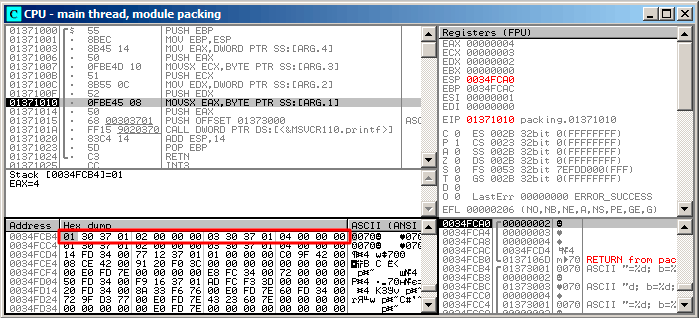
\includegraphics[scale=\FigScale]{patterns/15_structs/4_packing/olly_packing_4.png}
\caption{\olly: \RU{Перед исполнением \printf}\EN{Before \printf execution}}
\label{fig:packing_olly_4}
\end{figure}

\RU{В окне данных видим наши четыре поля}\EN{We see our 4 fields in the data window}.
\RU{Вот только, откуда взялись случайные байты (0x30, 0x37, 0x01) рядом с первым (a) и третьим (c) полем?}
\EN{But where do the random bytes (0x30, 0x37, 0x01) come from, that are next to the first (a) and third (c) fields?}
\RU{Если вернетесь к листингу \myref{src:struct_packing_4}, то увидите, что первое и третье поле имеет
тип \Tchar, а следовательно, туда записывается только один байт, 1 и 3 соответственно (строки 6 и 8).}
\EN{By looking at our listing \myref{src:struct_packing_4}, we can see that the first and third fields
are \Tchar, therefore only one byte is written, 1 and 3 respectively (lines 6 and 8).}
\RU{Остальные три байта 32-битного слова не будут модифицироваться в памяти!}
\EN{The remaining 3 bytes of the 32-bit words are not being modified in memory!}
\RU{А, следовательно, там остается случайный мусор.}\EN{Hence, random garbage is left there.}
\index{x86!\Instructions!MOVSX}
\RU{Этот мусор никак не будет влиять на работу \printf,
потому что значения для нее готовятся при помощи инструкции \MOVSX, которая загружает
из памяти байты а не слова}
\EN{This garbage doesn't influence the \printf output in any way, because the values for it are prepared
using the \MOVSX instruction, which takes bytes, but not words}: 
\lstref{src:struct_packing_4} (\RU{строки}\EN{lines} 34 \AndENRU 38).

\RU{Кстати, здесь используется именно \MOVSX (расширяющая знак), потому что тип 
\Tchar\EMDASH{}знаковый по умолчанию в MSVC и GCC.}
\EN{By the way, the \MOVSX (sign-extending) instruction is used here, because 
\Tchar is signed by default in MSVC and GCC.}
\RU{Если бы здесь был тип}\EN{If the type} \TT{unsigned char} \OrENRU \TT{uint8\_t}\EN{ was used here}, 
\RU{то здесь была бы инструкция \MOVZX}\EN{\MOVZX instruction would have been used instead}.

\clearpage
\subsubsection{\olly + \RU{упаковка полей по границе в 1 байт}\EN{fields aligning on 1 byte boundary}}
\index{\olly}

\RU{Здесь всё куда понятнее: 4 поля занимают 10 байт и значения сложены в памяти друг к другу}
\EN{Things are much clearer here: 4 fields occupy 10 bytes and the values are stored side-by-side}

\begin{figure}[H]
\centering
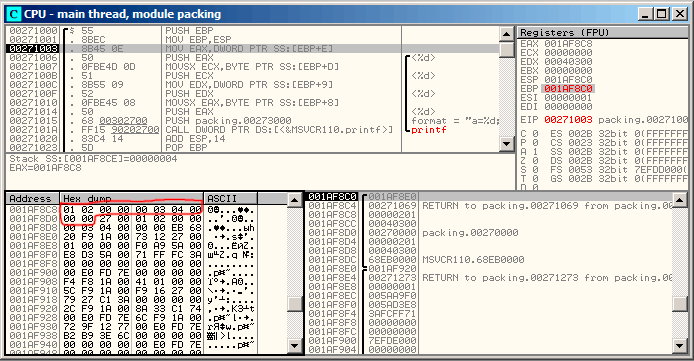
\includegraphics[scale=\FigScale]{patterns/15_structs/4_packing/olly_packing_1.png}
\caption{\olly: \RU{Перед исполнением \printf}\EN{Before \printf execution}}
\label{fig:packing_olly_1}
\end{figure}

\fi
